% Packages %%%%%%%%%%%%%%%%%%%%%%%%%%%%%%%%%%%%%%%%%%%%%%%%%%%
\documentclass[conference]{IEEEtran}
\IEEEoverridecommandlockouts 
\usepackage{cite}
\usepackage[cmex10]{amsmath}
\usepackage{amssymb}
%\usepackage{algorithmic}
\usepackage{array}
\usepackage{mdwmath}
\usepackage{mdwtab}
\usepackage{eqparbox}
\usepackage{graphicx}
\usepackage[]{subfigure}
\usepackage{url}
\usepackage[algoruled,vlined,linesnumbered]{algorithm2e}
\usepackage{verbatim}
\usepackage{color}
\usepackage{hyperref}
\usepackage{mathtools}

\makeindex 
\makeatletter

%%%%%%%%%%%%%%%%%%%%%%%%%%%%%%%%%%%%%%%%%%%%%%%%%%%%%%%%%%%%%%%%
% Magic stuff to shrink stuff
\makeatletter
\renewcommand\section{\@startsection{section}{1}{\z@}
                                  {-3.0ex plus -1.5ex minus -0.5ex}
                                  {0.7ex plus 1ex minus 0ex}
                                  {\bfseries}}
\renewcommand\subsection{\@startsection{subsection}{1}{\z@}
                                  {-2.0ex plus -1.5ex minus -0.5ex}
                                  {0.7ex plus 1ex minus 0ex}
                                  {\itshape\bfseries}}
\makeatother


%\newcommand{\shrinka}{\def\baselinestretch{0.99}\large\normalsize}

\long\def\IGNORE#1{}

%%%%%%%%%%%%%%%%%%%%%%%%%%%%%%%%%%%%%%%%%%%%%%%%%%%%%%%%%%%%%%%%%%%
% New commands
\newcommand{\Disks}{\ensuremath{\mathcal{D}}}
\newcommand{\Container}{\ensuremath{\mathit{C}}}
\newcommand{\initMax}{r_{0}\_\text{\textit{Max}}}
\newcommand{\initMin}{r_{0}\_\text{\textit{Min}}}

%%%%%%%%%%%%%%%%%%%%%%%%%%%%%%%%%%%%%%%%%%%%%%%%%%%%%%%%%%%%
% Paper Info
\author{ Ana Huam\'{a}n Quispe% <-this % stops a space
  \thanks{The author is with the Georgia Institute of Technology, Atlanta, GA.{\tt\small ahuaman3@gatech.edu}}}
\title{ {ECE8843} {A}ssignment 2 : {L}earning {R}obot {C}ontrol {S}trategies }  
%%%%%%%%%%%%%%%%%%%%%%%%%%%%%%%%%%%%%%%%%%%%%%%%%%%%%%%%%%%%
% Document
\begin{document}
\maketitle
%%%%%%%%%%%%%%%%%%%%%%%%%%%%%%%%%%%%%%%%%%%%%%%%%%%
%% Problem Statement
\section{Problem Statement}
Robby, the Soda-Can-Collecting robot has the job of cleaning up his  environment
by collecting soda cans. His gridded world is shown in Fig.\ref{fig:sodaCanMap}:

%------------------------------------------------------------
% Image: World Map
\begin{figure}[h]
	\centering
	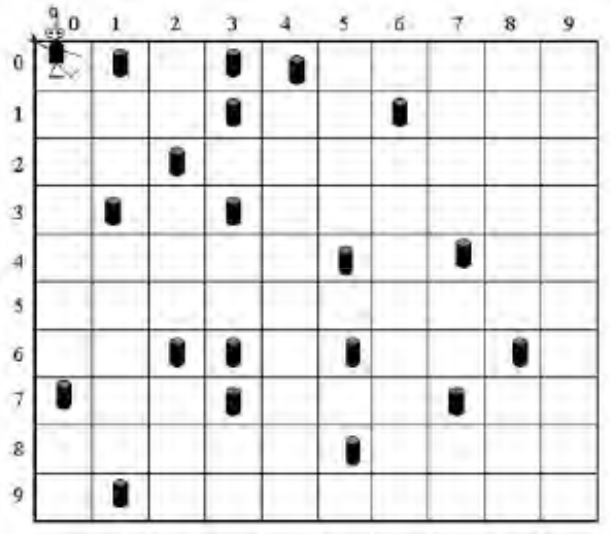
\includegraphics[width=0.9\columnwidth]{images/sodaCanMap.png} 
	\label{fig:sodaCanMap}
	\caption{$10\times10$ gridded world}
\end{figure}

% ********************
\subsection{Actions}
The robot has 7 possible actions:
\begin{itemize}
\item{\textit{North:} Move one grid up}
\item{\textit{South:} Move one grid down}
\item{\textit{East:} Move one grid right}
\item{\textit{West:} Move one grid left}
\item{\textit{Stay:} Stay on same location}
\item{\textit{Pick up:} Stay, bend and pick up can (if any)}
\item{\textit{Random:} Any of the above}
\end{itemize}

The number of allowed actions per episode is 200.

% ********************
\subsection{Rewards}
\begin{itemize}
\item{\textit{Move (North, South, East or West):} -1 }
\item{\textit{Bump wall:} -5}
\item{\textit{Failed pick up:} -2}
\item{\textit{Successful pick up:} +10}
\end{itemize}

% ********************
\subsection{States}
Robot states are composed of 5 variables, each of which
can have 3 possible values:
\begin{itemize}
\item{\textit{Current Grid:} Free, Can or Wall}
\item{\textit{North Grid:} Free, Can or Wall}
\item{\textit{South Grid:} Free, Can or Wall}
\item{\textit{East Grid:} Free, Can or Wall}
\item{\textit{West Grid:} Free, Can or Wall}
\end{itemize}

Having a total of $3^{5}=243$ states

%%%%%%%%%%%%%%%%%%%%%%%%%%%%%%%%%%%%%%%%%%%%%%%%%%%
%% Greedy Approach
\section{Greedy Approach}
We solved the problem
by using a simple variant of the well-known $\epsilon-\text{greedy}$ approach. 
At each time step, the robot has two possible ways to choose an action:
\begin{itemize}
\item{\textit{With probability $\epsilon$:} Choose a random action such that the
robot does not bump into walls (north, south,
east, west, stay or pick up)}
\item{\textit{With probability $1-\epsilon$:} Choose the action with highest reward,
that is:
	\begin{itemize}
	\item{If $\ArgSty{CURRENT\_GRID}$ is $\ArgSty{CAN}$ $\rightarrow$ Action is $\ArgSty{PICK\_UP}$}
	\item{Else \begin{itemize}
		\item{If $\ArgSty{NORTH\_GRID}$ is $\ArgSty{CAN}$ $\rightarrow$ Action is $\ArgSty{NORTH}$ }
		\item{If $\ArgSty{SOUTH\_GRID}$ is $\ArgSty{CAN}$ $\rightarrow$ Action is $\ArgSty{SOUTH}$ }
		\item{If $\ArgSty{EAST\_GRID}$ is $\ArgSty{CAN}$ $\rightarrow$ Action is $\ArgSty{EAST}$ }
		\item{If $\ArgSty{WEST\_GRID}$ is $\ArgSty{CAN}$ $\rightarrow$ Action is $\ArgSty{WEST}$ }		
		\item{Else $\rightarrow$ Action is $\ArgSty{RANDOM}$ }						
		\end{itemize}
	}
	\end{itemize}
}
\end{itemize}

Although fairly simple, this approach works
moderately well. Table \ref{tab:greedy} shows the results obtained in 10 runs of our program
with randomly generated starting positions:

%--------------------------------------------
% Table: Results with Greedy approach
\begin{table}[h]
\centering
\caption{Results of greedy approach ($\epsilon=0.05$)}
\begin{tabular}{|c|c|c|c|}
\hline 
\textit{ \textbf{Episode}} & \textit{ \textbf{Start Location}} & \textit{ \textbf{Final Value}} &  \textit{ \textbf{Cans Picked}}\\
\hline 
0 & $(3,1)$ & $-38$ & 15 \\
1 & $(0,2)$ & $-39$ & 15 \\
2 & $(8,3)$ & $6$ & 19 \\
3 & $(6,4)$ & $-35$ & 15 \\
4 & $(0,3)$ & $-58$ & 13 \\
5 & $(8,2)$ & $-62$ & 13 \\
6 & $(8,8)$ & $-17$ & 17 \\
7 & $(8,5)$ & $6$ & 19 \\
8 & $(1,3)$ & $-69$ & 12 \\ 
9 & $(8,4)$ & $-16$ & 17 \\ 
\hline
\end{tabular}
\label{tab:greedy}
\end{table} 

%%%%%%%%%%%%%%%%%%%%%%
\section{Sample Trial Run}
To exemplify the usefulness of our approach we provide the result of 01
run of our code. The output is attached on the zip file containing
this .pdf (name of the document is sampleRun.txt)

\end{document}